When working with Level Sets you almost always work with small objects
in a much bigger world. This is due to the fact that our level set is
defined in global space, and we have to manipulate it in the complete
workspace to make sure the SDF is always welldefined, meaning the
length of the gradient is equal to one. This is a time consuming
process as described in section \vref{sec:reinitialize}. A solution to
make the processes faster is to only work on the areas of the SDF just
beside the contour of the level set we are working on. This method is
called the Narrow Band method and is described
in \cit{adalsteinsson1995fast}. A Narrow band of the Aarhus University logo can be seen in figure \vref{fig:nb-au-logo}.


\begin{figure}[h]
  \centering
  \subfloat[The interface]{
    
\includegraphics[width=0.3\textwidth]{imgs/nb-au}}
  \subfloat[The Narrow band]{
    
\includegraphics[width=0.3\textwidth]{imgs/nb-au-band}}

  \caption{Visualizing the Narrow band of the AU logo.}
  \label{fig:nb-au-logo}
\end{figure}

\subsection*{Idea of the Narrow Band Method}
The basic idea of the method is to narrow down the amount of pixels we
are working on, to include as few as possible without loosing
precision. This is done by keeping a band of $\gamma$ pixels around
the edges in SDF so we only update the SDF where
$\gamma \leq \phi(x,y) \leq \gamma$. When we solve the level set
equation within the narrow band, we use the values of the neighboring
pixels and as we can't trust the pixels outside our narrow band, we
have to do this in another way. This is where the outer band, also
called an safety band, comes in to play. All the neighbors on both
sides of our narrow band is added to this set. The outer band only job
is to supply the inner band with information when calculating on the
border of the band. Because we know how big $\gamma$ is, it is safe to
assume that the distance from the outer band to $\phi=0$ is more or
less $\gamma$. Setting the value of all pixels in the outer band to
$\gamma$ is therefore safe if we promise to reinitialize the band
afterwards to make the length of the gradients to become 1 again. This
will make the whole narrow band including the outer band satisfy the
requirements of the SDF and we only have to do inside the band
itself. Hence the program flow is changed a little. We first advect
the interface by solving the level set equation on the SDF. We then
recalibrate the narrow band to fit the newly generated SDF and
then at the end reinitialize it.


\begin{figure}[!ht]
  \centering
  \begin{tabular}{ | c | }
   \hline			
   Solve level set equation \\
   \hline
   Update narrow band \\
   \hline   
   Reinitialize \\
   \hline  
  \end{tabular}
  \caption{Program flow with Narrow band}
  \label{fig:narrowband_flow}
\end{figure}


To decide the size of $\gamma$, and thereby the width of the narrow
band, we have to look at the maximum distance the interface can move
in a time step. In our implementation this boundary is at one pixel
per time step, therefor a narrow band of size 3 around the interface
is sufficient. As seen in figure \vref{fig:nb-au-logo} the band
reaches just outside the interface border as displayed in red. The
green outline around the red band is the outer safe band.

\begin{figure}[h]
  \centering
  \subfloat[The output]{
    
\includegraphics[width=0.3\textwidth]{imgs/nb1}}
  \subfloat[Without narrow band]{
    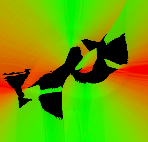
\includegraphics[width=0.3\textwidth]{imgs/nb2}}
  \subfloat[With narrow band]{
    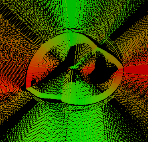
\includegraphics[width=0.3\textwidth]{imgs/nb3}}
  \caption{Same step while only reinitializing once per time step. Black in (b) and (c) represents an erroneous length of gradient.}
  \label{fig:narrowBand}
\end{figure}

As seen in figure \vref{fig:narrowBand}, the narrow band method is
powerful. Using the method we have significantly lowered the number of
pixels needed to visit while working with the SDF, simultaneously we
have reduced the number of times needed to reinitialize. If we only
reinitialize once it is clear that the method without narrow band is
more correct overall, though it contains large amounts of wrong data
around the interface, making calculations faulty. The narrow band
version is clearly wrong in the majority of the pixels, but around the
interface we see that the narrow band is in effect and the one
reinitialisation per time step almost covers our needs. 


\subsection{Implementation}
To represent our Narrow band we need a data structure to hold the new
information. Normally we traverse the workspace linearly and know
which pixels have been updated, and which we are going to visit
next. In the narrow band approach we have no linearity, the narrow
band can be divided into many detached objects in the
workspace. Therefore we need another way to traverse it than run
through (x,y) in the height and with of the workspace. Our solution is
to keep every pixel in a vector with (x,y) coordinates, and add the
vectors of the pixels inside the narrow band to a list. This list will
then contain the complete narrow band, both inner and outer band. To
distinct the two bands from each other we are using a 2D matrix
holding an 1 if the said pixel is in the inner band, and a 2 if it is
in the outer, 0 means the pixel is in neither. We also maintain an
integer containing the number of pixels inside the narrow band.

To build the narrow band, the technique is simply to traverse the SDF
and check the distance to an interface. If we within the $\gamma$
range of it, we are inside the narrow band, and the pixel is added to
the set of pixels inside the band. Meanwhile we add the said pixel to
the matrix telling which of the bands it is contained in. For
simplicity we can in the same traversal check if it should be in the
outer band if it isn't inside the inner band. As it does not matter if
we take too much in the outer band, we here just check if it is in
$\gamma$ range + 2 pixel. We take more than needed, but we are on the
safe side. The type of the pixels in the outer band is of course added
to the type matrix. This is done as shown by this code stump:

%\subsection{Building the initial narrow band}
\begin{lstlisting}
    for (unsigned int x=0; x<width; x++)
        for (unsigned int y=0; y<height; y++) {
            float phiVal = fabs((*phi)(x, y));
            if (phiVal <= narrowBandWidth) {
                //Part of the inner band
                narrowBand[narrowBandSize++] = (Vector<2,int> (x,y));
                nbType(x,y) = 1;
            } else if (phiVal <= narrowBandWidth + 2.0f) {
                //Part of the outer(safety) band
                narrowBand[narrowBandSize++] = (Vector<2,int> (x,y));
                nbType(x,y) = 2;
            } else {
                nbType(x,y) = 0;
            }
        }
\end{lstlisting}


\subsection{Rebuilding the narrow band}
As we have defined a narrow band to work inside, it seems odd to
rebuild this every time step by traversing the entire
workspace. In \cit{peng1999pde} is described a solution where the
rebuilding time of the narrow band has been optimized. We again use
the fact we know our interface only can move 1 pixel per time step,
hence our new inner band must be within the old narrow band. Knowing
this we only need to traverse the old narrow band to see which pixels
are within $\gamma$ distance of our new interface position. Whilst
doing this we also update the type matrix, removing the pixels now no
more resides inside a band. Now the tricky part comes; finding the
outer band. This can be done in a separate step, where we traverse the
new inner band, and for each pixel visits the neighbors. If the
neighbor is set to 0 in the type matrix, we change it to 2, and add it
to the end of our narrow band list. Many of the visited pixels will
already be inside the narrow band, but the time spared not traversing
the entire workspace is worth it. 


                %% if ((*phi)(x,y) >= 0)
                %%     (*phi)(x,y) = narrowBandWidth;
                %% else 
                %%     (*phi)(x,y) = -narrowBandWidth;



\subsection{Conclusion}
\todoVester[inline]{Skriv NB Conclution}
